\section{Simulation des fonctions}

\subsection{Interface Microprocesseur}

Dans cette section, nous présentons la simulation du bloc \textit{Interface Microprocesseur} et l’analyse des chronogrammes obtenus.  
La simulation a été réalisée à l’aide d’un \textit{testbench}, implémenté sous la forme d’un bloc nommé \texttt{EnvTest\_InterfaceMicroprocesseur}, connecté au composant \texttt{InterfaceMicroprocesseur}.  
L’objectif est de vérifier la conformité du fonctionnement par rapport à l’automate décrit dans la section \textit{Architecture}.

\begin{figure}[H]
    \centering
    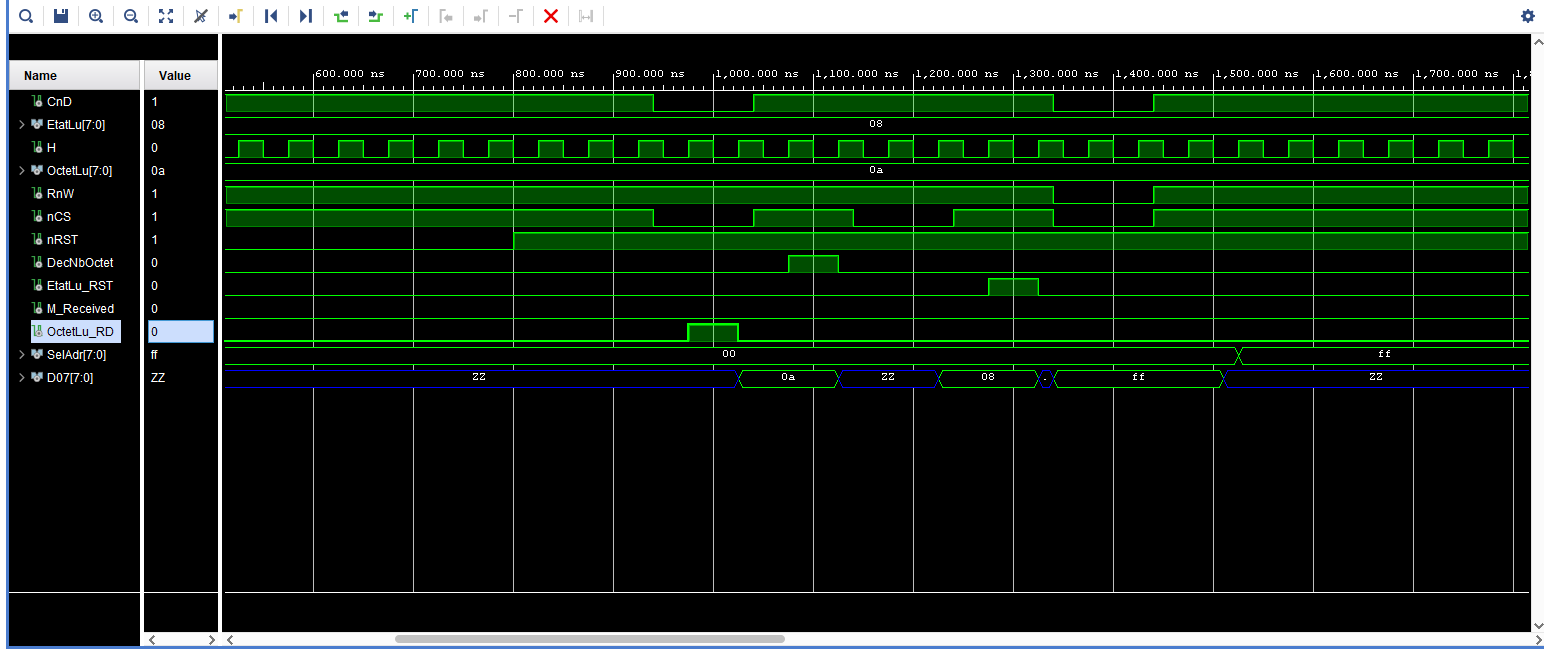
\includegraphics[width=0.95\linewidth]{images//Simulation/Chrono.png}
    \caption{Chronogramme de simulation de l’Interface Microprocesseur}
    \label{fig:placeholder}
\end{figure}

Le testbench (fourni en annexe) a pour rôle de reproduire l’environnement dans lequel le composant est amené à fonctionner.  
Il émule le comportement d’un microprocesseur en générant automatiquement les stimuli nécessaires à la validation du bloc testé.

\subsubsection{Déclarations et signaux}
Le testbench commence par la déclaration des librairies \texttt{IEEE}, nécessaires à la manipulation des types logiques et des vecteurs binaires.  
Les principaux signaux utilisés sont :
\begin{itemize}
  \item \texttt{CnD}, \texttt{RnW}, \texttt{nCS}, \texttt{nRST}, \texttt{H} : lignes de contrôle classiques d’une interface microprocesseur (commande/données, lecture/écriture, sélection du composant, reset, horloge),
  \item \texttt{OctetLu}, \texttt{EtatLu}, \texttt{SelAdr}, \texttt{D07} : bus de données et d’adresses sur 8 bits,
  \item \texttt{DecNbOctet}, \texttt{EtatLu\_RST}, \texttt{M\_Received}, \texttt{OctetLu\_RD} : signaux internes utilisés pour la communication avec le composant testé.
\end{itemize}

\subsubsection{Instanciation du composant testé}
Le composant \texttt{InterfaceMicroprocesseur} est instancié dans l’architecture de simulation.  
Il est relié à l’ensemble des signaux déclarés, permettant ainsi l’observation de son comportement face aux stimuli générés.

\subsubsection{Environnement de test}
Le composant \texttt{EnvTest\_InterfaceMicroprocesseur} simule le rôle du microprocesseur en générant automatiquement les signaux nécessaires :
\begin{itemize}
  \item génération de l’horloge (\texttt{H}),
  \item gestion du reset global (\texttt{nRST}),
  \item activation des commandes de lecture/écriture (\texttt{RnW}, \texttt{CnD}, \texttt{nCS}),
  \item pilotage du bus de données (\texttt{D07}).
\end{itemize}

Cet environnement est paramétré par plusieurs génériques :
\begin{itemize}
  \item \texttt{CLOCK\_PERIOD} : période d’horloge (50 ns),
  \item \texttt{RESET\_OFFSET} et \texttt{RESET\_DURATION} : moment et durée du reset (500 ns et 300 ns),
  \item \texttt{ACCESS\_TIME} et \texttt{HOLD\_TIME} : contraintes temporelles d’accès et de maintien (40 ns et 70 ns).
\end{itemize}

\begin{figure}[H]
    \centering
    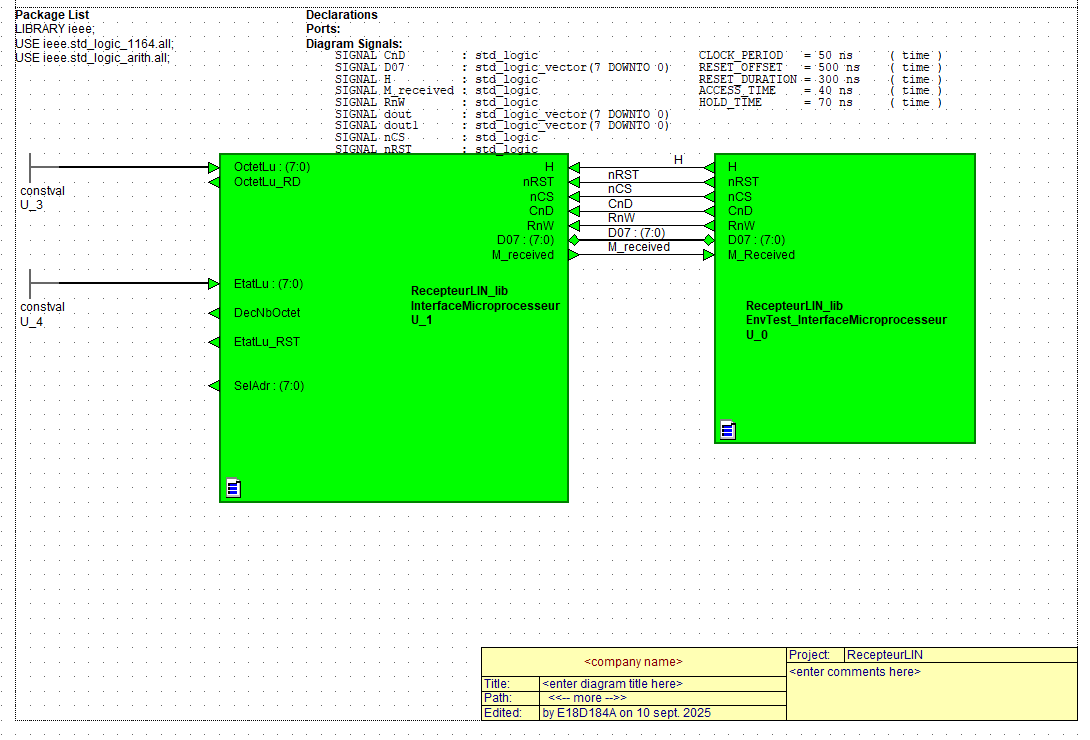
\includegraphics[width=0.95\linewidth]{images/Simulation/banc_test.png}
    \caption{Block Diagramme de test de l’Interface Microprocesseur}
    \label{fig:placeholder}
\end{figure}

\subsubsection{Stimuli supplémentaires}
Un processus spécifique (\texttt{StimProc}) complète la génération des signaux.  
Après la fin du reset, il impose des valeurs constantes sur certaines lignes :
\begin{itemize}
  \item \texttt{OctetLu} $\leftarrow$ 10 (codé sur 8 bits),
  \item \texttt{EtatLu} $\leftarrow$ 8 (codé sur 8 bits).
\end{itemize}
Ces valeurs permettent de vérifier la gestion correcte des données reçues par l’interface.  
La simulation est ensuite maintenue en attente infinie.

\subsubsection{Analyse du chronogramme de simulation}
L’analyse du chronogramme met en évidence le comportement attendu du composant :
\begin{itemize}
  \item lorsque les signaux de contrôle actifs à l’état bas (\texttt{nRST}, \texttt{nCS}) sont à l’état haut, aucune action n’est effectuée,
  \item lorsque ces signaux sont activés (passage à l’état bas), le composant réagit conformément à l’automate interne,
  \item les signaux \texttt{RnW} et \texttt{CnD} permettent de sélectionner respectivement les opérations de lecture/écriture et le type d’accès (commande ou données),
  \item les valeurs imposées sur \texttt{OctetLu} et \texttt{EtatLu} sont correctement lues via le bus de données \texttt{D07}.
\end{itemize}

Ce chronogramme confirme ainsi le bon fonctionnement du composant \texttt{InterfaceMicroprocesseur} :  
après la levée du reset, l’environnement de test génère des cycles de lecture et d’écriture auxquels le composant répond correctement, en échangeant les données prévues et en activant les signaux de contrôle appropriés.
